\section{FHT Class Reference}
\label{classFHT}\index{FHT@{FHT}}
{\tt \#include $<$fht.h$>$}



\subsection{Detailed Description}
Implementation of the Hartley Transform after Bracewell's discrete algorithm. The algorithm is subject to US patent No. 4,646,256 (1987) but was put into public domain by the Board of Trustees of Stanford University in 1994 and is now freely available[1].

[1] Computer in Physics, Vol. 9, No. 4, Jul/Aug 1995 pp 373-379 



Definition at line 32 of file fht.h.\subsection*{Public Member Functions}
\begin{CompactItemize}
\item 
{\bf FHT} (int)
\item 
{\bf $\sim$FHT} ()
\item 
int {\bf size\-Exp} () const 
\item 
int {\bf size} () const 
\item 
float $\ast$ {\bf copy} (float $\ast$, float $\ast$)
\item 
float $\ast$ {\bf clear} (float $\ast$)
\item 
void {\bf scale} (float $\ast$, float)
\item 
void {\bf ewma} (float $\ast$d, float $\ast$s, float w)
\item 
void {\bf pattern} (float $\ast$d, bool rect)
\item 
void {\bf log\-Spectrum} (float $\ast$out, float $\ast$p)
\item 
void {\bf semi\-Log\-Spectrum} (float $\ast$)
\item 
void {\bf spectrum} (float $\ast$)
\item 
void {\bf power} (float $\ast$)
\item 
void {\bf power2} (float $\ast$)
\item 
void {\bf transform8} (float $\ast$)
\item 
void {\bf transform} (float $\ast$)
\end{CompactItemize}
\subsection*{Private Member Functions}
\begin{CompactItemize}
\item 
void {\bf make\-Cas\-Table} ()
\item 
void {\bf \_\-transform} (float $\ast$, int, int)
\end{CompactItemize}
\subsection*{Private Attributes}
\begin{CompactItemize}
\item 
int {\bf m\_\-exp2}
\item 
int {\bf m\_\-num}
\item 
float $\ast$ {\bf m\_\-buf}
\item 
float $\ast$ {\bf m\_\-tab}
\item 
int $\ast$ {\bf m\_\-log}
\end{CompactItemize}


\subsection{Constructor \& Destructor Documentation}
\index{FHT@{FHT}!FHT@{FHT}}
\index{FHT@{FHT}!FHT@{FHT}}
\subsubsection{\setlength{\rightskip}{0pt plus 5cm}FHT::FHT (int)}\label{classFHT_FHTa0}


Prepare transform for data sets with $2^n$ numbers, whereby $n$ should be at least 3. Values of more than 3 need a trigonometry table. \begin{Desc}
\item[See also:]{\bf make\-Cas\-Table()}{\rm (p.\,\pageref{classFHT_FHTd0})}\end{Desc}


Definition at line 26 of file fht.cpp.

References m\_\-buf, m\_\-exp2, m\_\-num, m\_\-tab, and make\-Cas\-Table().



\footnotesize\begin{verbatim}26               :
27         m_buf(0),
28         m_tab(0),
29         m_log(0)
30 {
31         if (n < 3) {
32                 m_num = 0;
33                 m_exp2 = -1;
34                 return;
35         }
36         m_exp2 = n;
37         m_num = 1 << n;
38         if (n > 3) {
39                 m_buf = new float[m_num];
40                 m_tab = new float[m_num * 2];
41                 makeCasTable();
42         }
43 }

\end{verbatim}\normalsize 


Here is the call graph for this function:\begin{figure}[H]
\begin{center}
\leavevmode
\includegraphics[width=120pt]{classFHT_FHTa0_cgraph}
\end{center}
\end{figure}
\index{FHT@{FHT}!~FHT@{$\sim$FHT}}
\index{~FHT@{$\sim$FHT}!FHT@{FHT}}
\subsubsection{\setlength{\rightskip}{0pt plus 5cm}FHT::$\sim${\bf FHT} ()}\label{classFHT_FHTa1}




Definition at line 46 of file fht.cpp.

References m\_\-buf, m\_\-log, and m\_\-tab.



\footnotesize\begin{verbatim}47 {
48         delete[] m_buf;
49         delete[] m_tab;
50         delete[] m_log;
51 }
\end{verbatim}\normalsize 


\subsection{Member Function Documentation}
\index{FHT@{FHT}!_transform@{\_\-transform}}
\index{_transform@{\_\-transform}!FHT@{FHT}}
\subsubsection{\setlength{\rightskip}{0pt plus 5cm}void FHT::\_\-transform (float $\ast$, int, int)\hspace{0.3cm}{\tt  [private]}}\label{classFHT_FHTd1}


Recursive in-place Hartley transform. For internal use only!

Definition at line 221 of file fht.cpp.

References m\_\-buf, m\_\-num, m\_\-tab, and transform8().

Referenced by power2(), and transform().



\footnotesize\begin{verbatim}222 {
223         if (n == 8) {
224                 transform8(p + k);
225                 return;
226         }
227 
228         int i, j, ndiv2 = n / 2;
229         float a, *t1, *t2, *t3, *t4, *ptab, *pp;
230 
231         for (i = 0, t1 = m_buf, t2 = m_buf + ndiv2, pp = &p[k]; i < ndiv2; i++)
232                 *t1++ = *pp++, *t2++ = *pp++;
233 
234         memcpy(p + k, m_buf, sizeof(float) * n);
235 
236         _transform(p, ndiv2, k);
237         _transform(p, ndiv2, k + ndiv2);
238 
239         j = m_num / ndiv2 - 1;
240         t1 = m_buf;
241         t2 = t1 + ndiv2;
242         t3 = p + k + ndiv2;
243         ptab = m_tab;
244         pp = p + k;
245 
246         a = *ptab++ * *t3++;
247         a += *ptab * *pp;
248         ptab += j;
249 
250         *t1++ = *pp + a;
251         *t2++ = *pp++ - a;
252 
253         for (i = 1, t4 = p + k + n; i < ndiv2; i++, ptab += j) {
254                 a = *ptab++ * *t3++;
255                 a += *ptab * *--t4;
256 
257                 *t1++ = *pp + a;
258                 *t2++ = *pp++ - a;
259         }
260         memcpy(p + k, m_buf, sizeof(float) * n);
261 }
\end{verbatim}\normalsize 


Here is the call graph for this function:\begin{figure}[H]
\begin{center}
\leavevmode
\includegraphics[width=126pt]{classFHT_FHTd1_cgraph}
\end{center}
\end{figure}
\index{FHT@{FHT}!clear@{clear}}
\index{clear@{clear}!FHT@{FHT}}
\subsubsection{\setlength{\rightskip}{0pt plus 5cm}float $\ast$ FHT::clear (float $\ast$)}\label{classFHT_FHTa5}




Definition at line 76 of file fht.cpp.

References m\_\-num.



\footnotesize\begin{verbatim}77 {
78         return (float *)memset(d, 0, m_num * sizeof(float));
79 }
\end{verbatim}\normalsize 
\index{FHT@{FHT}!copy@{copy}}
\index{copy@{copy}!FHT@{FHT}}
\subsubsection{\setlength{\rightskip}{0pt plus 5cm}float $\ast$ FHT::copy (float $\ast$, float $\ast$)}\label{classFHT_FHTa4}




Definition at line 70 of file fht.cpp.

References m\_\-num.

Referenced by Analyzer::Base$<$ W $>$::transform().



\footnotesize\begin{verbatim}71 {
72         return (float *)memcpy(d, s, m_num * sizeof(float));
73 }
\end{verbatim}\normalsize 
\index{FHT@{FHT}!ewma@{ewma}}
\index{ewma@{ewma}!FHT@{FHT}}
\subsubsection{\setlength{\rightskip}{0pt plus 5cm}void FHT::ewma (float $\ast$ {\em d}, float $\ast$ {\em s}, float {\em w})}\label{classFHT_FHTa7}


Exponentially Weighted Moving Average (EWMA) filter. \begin{Desc}
\item[Parameters:]
\begin{description}
\item[{\em d}]is the filtered data. \item[{\em s}]is fresh input. \item[{\em w}]is the weighting factor.\end{description}
\end{Desc}


Definition at line 89 of file fht.cpp.

References m\_\-num.



\footnotesize\begin{verbatim}90 {
91         for (int i = 0; i < (m_num / 2); i++, d++, s++)
92                 *d = *d * w + *s * (1 - w);
93 }
\end{verbatim}\normalsize 
\index{FHT@{FHT}!logSpectrum@{logSpectrum}}
\index{logSpectrum@{logSpectrum}!FHT@{FHT}}
\subsubsection{\setlength{\rightskip}{0pt plus 5cm}void FHT::log\-Spectrum (float $\ast$ {\em out}, float $\ast$ {\em p})}\label{classFHT_FHTa9}


Logarithmic audio spectrum. Maps semi-logarithmic spectrum to logarithmic frequency scale, interpolates missing values. A logarithmic index map is calculated at the first run only. \begin{Desc}
\item[Parameters:]
\begin{description}
\item[{\em p}]is the input array. \item[{\em out}]is the spectrum.\end{description}
\end{Desc}


Definition at line 116 of file fht.cpp.

References m\_\-log, m\_\-num, and semi\-Log\-Spectrum().

Referenced by Analyzer::Base$<$ W $>$::transform().



\footnotesize\begin{verbatim}117 {
118         int n = m_num / 2, i, j, k, *r;
119         if (!m_log) {
120                 m_log = new int[n];
121                 float f = n / log10(n);
122                 for (i = 0, r = m_log; i < n; i++, r++) {
123                         j = int(rint(log10(i + 1.0) * f));
124                         *r = j >= n ? n - 1 : j;
125                 }
126         }
127         semiLogSpectrum(p);
128         *out++ = *p = *p / 100;
129         for (k = i = 1, r = m_log; i < n; i++) {
130                 j = *r++;
131                 if (i == j)
132                         *out++ = p[i];
133                 else {
134                         float base = p[k - 1];
135                         float step = (p[j] - base) / (j - (k - 1));
136                         for (float corr = 0; k <= j; k++, corr += step)
137                                 *out++ = base + corr;
138                 }
139         }
140 }
\end{verbatim}\normalsize 


Here is the call graph for this function:\begin{figure}[H]
\begin{center}
\leavevmode
\includegraphics[width=327pt]{classFHT_FHTa9_cgraph}
\end{center}
\end{figure}
\index{FHT@{FHT}!makeCasTable@{makeCasTable}}
\index{makeCasTable@{makeCasTable}!FHT@{FHT}}
\subsubsection{\setlength{\rightskip}{0pt plus 5cm}void FHT::make\-Cas\-Table ()\hspace{0.3cm}{\tt  [private]}}\label{classFHT_FHTd0}


Create a table of CAS (cosine and sine) values. Has only to be done in the constructor and saves from calculating the same values over and over while transforming.

Definition at line 54 of file fht.cpp.

References m\_\-num, and m\_\-tab.

Referenced by FHT().



\footnotesize\begin{verbatim}55 {
56         float d, *costab, *sintab;
57         int ul, ndiv2 = m_num / 2;
58 
59         for (costab = m_tab, sintab = m_tab + m_num / 2 + 1, ul = 0; ul < m_num; ul++) {
60                 d = M_PI * ul / ndiv2;
61                 *costab = *sintab = cos(d);
62 
63                 costab += 2, sintab += 2;
64                 if (sintab > m_tab + m_num * 2)
65                         sintab = m_tab + 1;
66         }
67 }
\end{verbatim}\normalsize 
\index{FHT@{FHT}!pattern@{pattern}}
\index{pattern@{pattern}!FHT@{FHT}}
\subsubsection{\setlength{\rightskip}{0pt plus 5cm}void FHT::pattern (float $\ast$ {\em d}, bool {\em rect})}\label{classFHT_FHTa8}


Test routine to create wobbling sine or rectangle wave. \begin{Desc}
\item[Parameters:]
\begin{description}
\item[{\em d}]destination vector. \item[{\em rect}]rectangle if true, sine otherwise.\end{description}
\end{Desc}


Definition at line 97 of file fht.cpp.

References m\_\-num, and sind().



\footnotesize\begin{verbatim}98 {
99         static float f = 1.0;
100         static float h = 0.1;
101         int i;
102         for (i = 0; i < 3 * m_num / 4; i++, p++) {
103                 float o = 360.0 * i / m_num;
104                 *p = sind(f * o);
105                 if (rect)
106                         *p = *p < 0 ? -1.0 : 1.0;
107         }
108         for (; i < m_num; i++)
109                 *p++ = 0.0;
110         if (f > m_num / 2.0 || f < .05)
111                 h = -h;
112         f += h;
113 }
\end{verbatim}\normalsize 


Here is the call graph for this function:\begin{figure}[H]
\begin{center}
\leavevmode
\includegraphics[width=90pt]{classFHT_FHTa8_cgraph}
\end{center}
\end{figure}
\index{FHT@{FHT}!power@{power}}
\index{power@{power}!FHT@{FHT}}
\subsubsection{\setlength{\rightskip}{0pt plus 5cm}void FHT::power (float $\ast$)}\label{classFHT_FHTa12}


Calculates a mathematically correct FFT power spectrum. If further scaling is applied later, use power2 instead and factor the 0.5 in the final scaling factor. \begin{Desc}
\item[See also:]{\bf FHT::power2()}{\rm (p.\,\pageref{classFHT_FHTa13})}\end{Desc}


Definition at line 162 of file fht.cpp.

References m\_\-num, and power2().

Referenced by Sonogram::transform().



\footnotesize\begin{verbatim}163 {
164         power2(p);
165         for (int i = 0; i < (m_num / 2); i++)
166                 *p++ *= .5;
167 }
\end{verbatim}\normalsize 


Here is the call graph for this function:\begin{figure}[H]
\begin{center}
\leavevmode
\includegraphics[width=233pt]{classFHT_FHTa12_cgraph}
\end{center}
\end{figure}
\index{FHT@{FHT}!power2@{power2}}
\index{power2@{power2}!FHT@{FHT}}
\subsubsection{\setlength{\rightskip}{0pt plus 5cm}void FHT::power2 (float $\ast$)}\label{classFHT_FHTa13}


Calculates an FFT power spectrum with doubled values as a result. The values need to be multiplied by 0.5 to be exact. Note that you only get $2^{n-1}$ power values for a data set of $2^n$ input values. \begin{Desc}
\item[See also:]{\bf FHT::power()}{\rm (p.\,\pageref{classFHT_FHTa12})}\end{Desc}


Definition at line 170 of file fht.cpp.

References \_\-transform(), and m\_\-num.

Referenced by power(), semi\-Log\-Spectrum(), and spectrum().



\footnotesize\begin{verbatim}171 {
172         int i;
173         float *q;
174         _transform(p, m_num, 0);
175 
176         *p = (*p * *p), *p += *p, p++;
177 
178         for (i = 1, q = p + m_num - 2; i < (m_num / 2); i++, --q)
179                 *p++ = (*p * *p) + (*q * *q);
180 }
\end{verbatim}\normalsize 


Here is the call graph for this function:\begin{figure}[H]
\begin{center}
\leavevmode
\includegraphics[width=181pt]{classFHT_FHTa13_cgraph}
\end{center}
\end{figure}
\index{FHT@{FHT}!scale@{scale}}
\index{scale@{scale}!FHT@{FHT}}
\subsubsection{\setlength{\rightskip}{0pt plus 5cm}void FHT::scale (float $\ast$, float)}\label{classFHT_FHTa6}




Definition at line 82 of file fht.cpp.

References m\_\-num.

Referenced by Sonogram::transform(), and Analyzer::Base$<$ W $>$::transform().



\footnotesize\begin{verbatim}83 {
84         for (int i = 0; i < (m_num / 2); i++)
85                 *p++ *= d;
86 }
\end{verbatim}\normalsize 
\index{FHT@{FHT}!semiLogSpectrum@{semiLogSpectrum}}
\index{semiLogSpectrum@{semiLogSpectrum}!FHT@{FHT}}
\subsubsection{\setlength{\rightskip}{0pt plus 5cm}void FHT::semi\-Log\-Spectrum (float $\ast$)}\label{classFHT_FHTa10}


Semi-logarithmic audio spectrum.

Definition at line 143 of file fht.cpp.

References m\_\-num, and power2().

Referenced by log\-Spectrum().



\footnotesize\begin{verbatim}144 {
145         float e;
146         power2(p);
147         for (int i = 0; i < (m_num / 2); i++, p++) {
148                 e = 10.0 * log10(sqrt(*p * .5));
149                 *p = e < 0 ? 0 : e;
150         }
151 }
\end{verbatim}\normalsize 


Here is the call graph for this function:\begin{figure}[H]
\begin{center}
\leavevmode
\includegraphics[width=260pt]{classFHT_FHTa10_cgraph}
\end{center}
\end{figure}
\index{FHT@{FHT}!size@{size}}
\index{size@{size}!FHT@{FHT}}
\subsubsection{\setlength{\rightskip}{0pt plus 5cm}int FHT::size () const\hspace{0.3cm}{\tt  [inline]}}\label{classFHT_FHTa3}




Definition at line 62 of file fht.h.

References m\_\-num.

Referenced by Sonogram::demo(), and Analyzer::Base$<$ W $>$::transform().



\footnotesize\begin{verbatim}62 { return m_num; }
\end{verbatim}\normalsize 
\index{FHT@{FHT}!sizeExp@{sizeExp}}
\index{sizeExp@{sizeExp}!FHT@{FHT}}
\subsubsection{\setlength{\rightskip}{0pt plus 5cm}int FHT::size\-Exp () const\hspace{0.3cm}{\tt  [inline]}}\label{classFHT_FHTa2}




Definition at line 61 of file fht.h.

References m\_\-exp2.



\footnotesize\begin{verbatim}61 { return m_exp2; }
\end{verbatim}\normalsize 
\index{FHT@{FHT}!spectrum@{spectrum}}
\index{spectrum@{spectrum}!FHT@{FHT}}
\subsubsection{\setlength{\rightskip}{0pt plus 5cm}void FHT::spectrum (float $\ast$)}\label{classFHT_FHTa11}


Fourier spectrum.

Definition at line 154 of file fht.cpp.

References m\_\-num, and power2().



\footnotesize\begin{verbatim}155 {
156         power2(p);
157         for (int i = 0; i < (m_num / 2); i++, p++)
158                 *p = (float)sqrt(*p * .5);
159 }
\end{verbatim}\normalsize 


Here is the call graph for this function:\begin{figure}[H]
\begin{center}
\leavevmode
\includegraphics[width=240pt]{classFHT_FHTa11_cgraph}
\end{center}
\end{figure}
\index{FHT@{FHT}!transform@{transform}}
\index{transform@{transform}!FHT@{FHT}}
\subsubsection{\setlength{\rightskip}{0pt plus 5cm}void FHT::transform (float $\ast$)}\label{classFHT_FHTa15}




Definition at line 183 of file fht.cpp.

References \_\-transform(), m\_\-num, and transform8().



\footnotesize\begin{verbatim}184 {
185         if (m_num == 8)
186                 transform8(p);
187         else
188                 _transform(p, m_num, 0);
189 }
\end{verbatim}\normalsize 


Here is the call graph for this function:\begin{figure}[H]
\begin{center}
\leavevmode
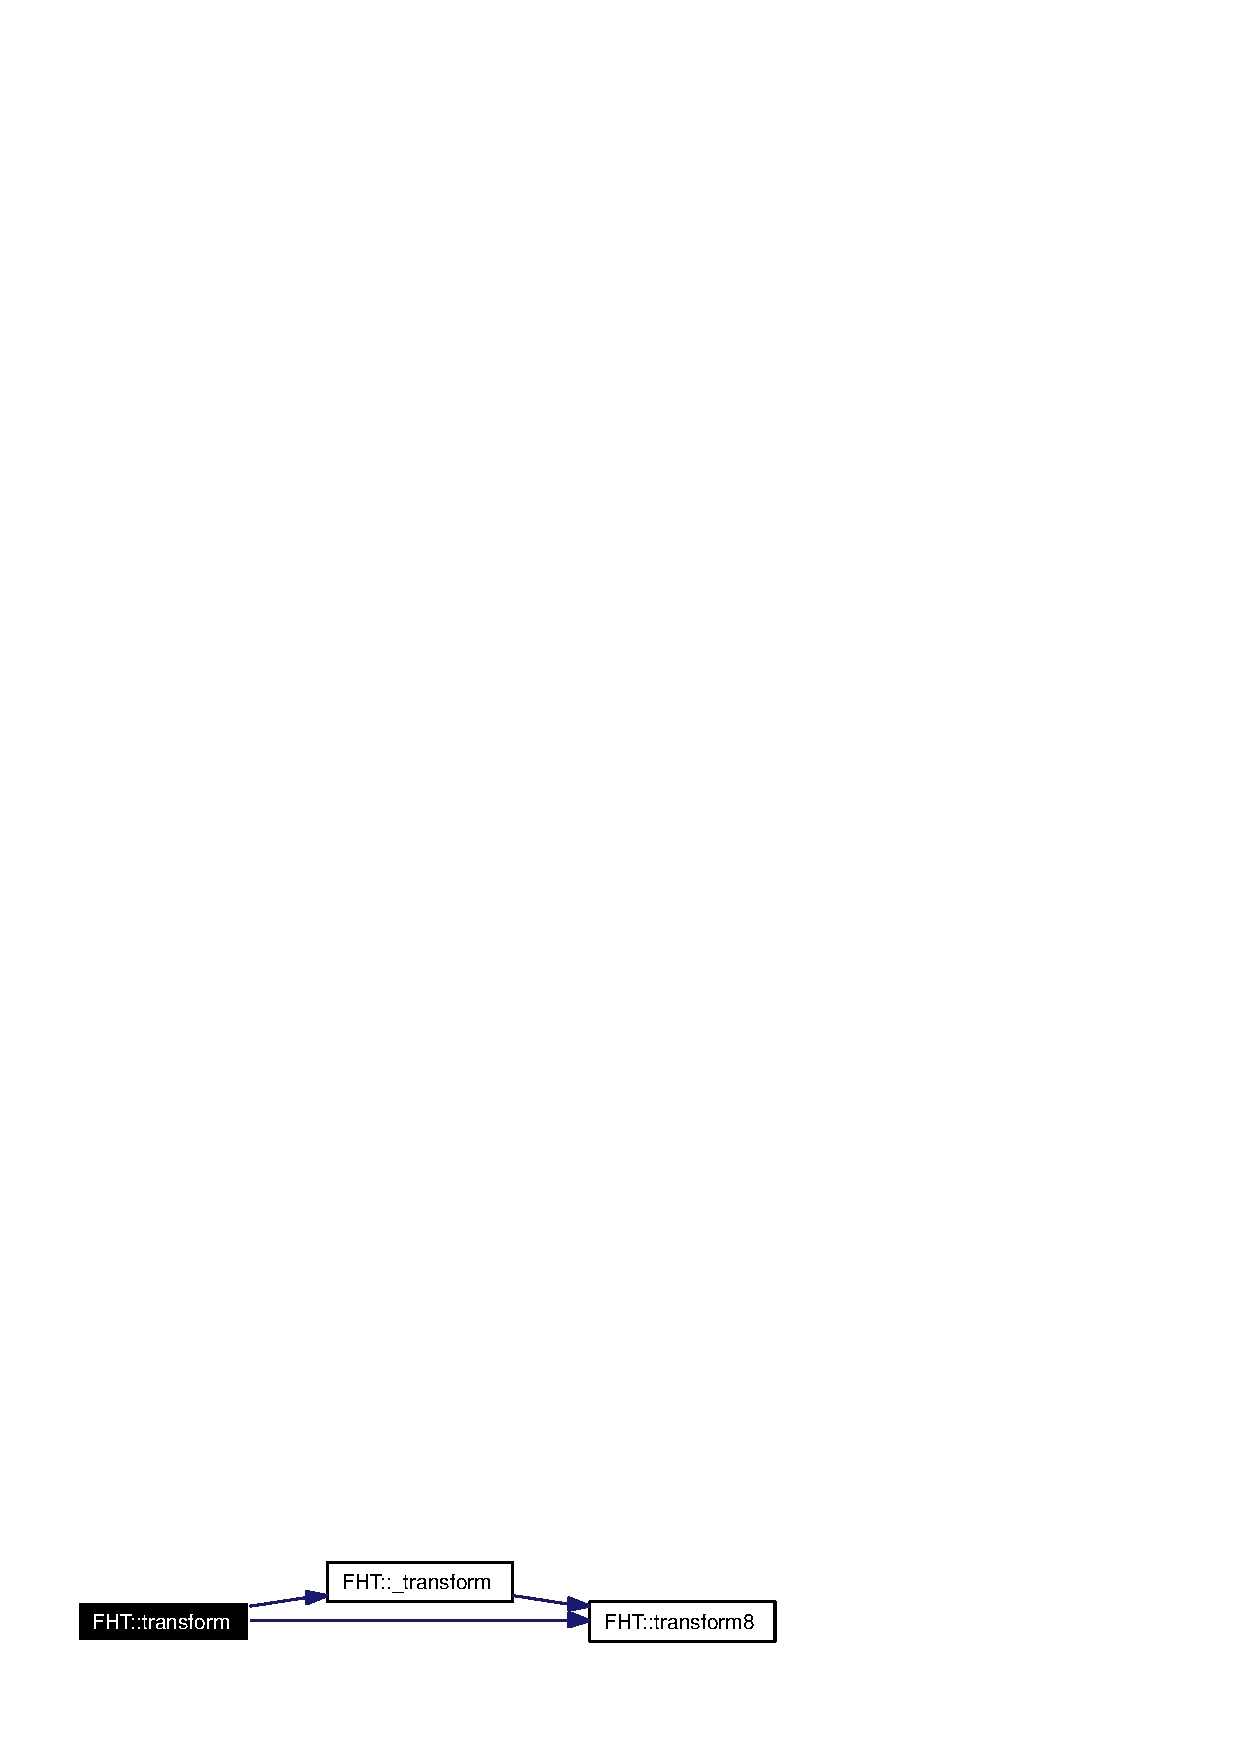
\includegraphics[width=186pt]{classFHT_FHTa15_cgraph}
\end{center}
\end{figure}
\index{FHT@{FHT}!transform8@{transform8}}
\index{transform8@{transform8}!FHT@{FHT}}
\subsubsection{\setlength{\rightskip}{0pt plus 5cm}void FHT::transform8 (float $\ast$)}\label{classFHT_FHTa14}


Discrete Hartley transform of data sets with 8 values.

Definition at line 192 of file fht.cpp.

Referenced by \_\-transform(), and transform().



\footnotesize\begin{verbatim}193 {
194         float a, b, c, d, e, f, g, h, b_f2, d_h2;
195         float a_c_eg, a_ce_g, ac_e_g, aceg, b_df_h, bdfh;
196 
197         a = *p++, b = *p++, c = *p++, d = *p++;
198         e = *p++, f = *p++, g = *p++, h = *p;
199         b_f2 = (b - f) * M_SQRT2;
200         d_h2 = (d - h) * M_SQRT2;
201 
202         a_c_eg = a - c - e + g;
203         a_ce_g = a - c + e - g;
204         ac_e_g = a + c - e - g;
205         aceg = a + c + e + g;
206 
207         b_df_h = b - d + f - h;
208         bdfh = b + d + f + h;
209 
210         *p = a_c_eg - d_h2;
211         *--p = a_ce_g - b_df_h;
212         *--p = ac_e_g - b_f2;
213         *--p = aceg - bdfh;
214         *--p = a_c_eg + d_h2;
215         *--p = a_ce_g + b_df_h;
216         *--p = ac_e_g + b_f2;
217         *--p = aceg + bdfh;
218 }
\end{verbatim}\normalsize 


\subsection{Member Data Documentation}
\index{FHT@{FHT}!m_buf@{m\_\-buf}}
\index{m_buf@{m\_\-buf}!FHT@{FHT}}
\subsubsection{\setlength{\rightskip}{0pt plus 5cm}float$\ast$ {\bf FHT::m\_\-buf}\hspace{0.3cm}{\tt  [private]}}\label{classFHT_FHTr2}




Definition at line 36 of file fht.h.

Referenced by \_\-transform(), FHT(), and $\sim$FHT().\index{FHT@{FHT}!m_exp2@{m\_\-exp2}}
\index{m_exp2@{m\_\-exp2}!FHT@{FHT}}
\subsubsection{\setlength{\rightskip}{0pt plus 5cm}int {\bf FHT::m\_\-exp2}\hspace{0.3cm}{\tt  [private]}}\label{classFHT_FHTr0}




Definition at line 34 of file fht.h.

Referenced by FHT(), and size\-Exp().\index{FHT@{FHT}!m_log@{m\_\-log}}
\index{m_log@{m\_\-log}!FHT@{FHT}}
\subsubsection{\setlength{\rightskip}{0pt plus 5cm}int$\ast$ {\bf FHT::m\_\-log}\hspace{0.3cm}{\tt  [private]}}\label{classFHT_FHTr4}




Definition at line 38 of file fht.h.

Referenced by log\-Spectrum(), and $\sim$FHT().\index{FHT@{FHT}!m_num@{m\_\-num}}
\index{m_num@{m\_\-num}!FHT@{FHT}}
\subsubsection{\setlength{\rightskip}{0pt plus 5cm}int {\bf FHT::m\_\-num}\hspace{0.3cm}{\tt  [private]}}\label{classFHT_FHTr1}




Definition at line 35 of file fht.h.

Referenced by \_\-transform(), clear(), copy(), ewma(), FHT(), log\-Spectrum(), make\-Cas\-Table(), pattern(), power(), power2(), scale(), semi\-Log\-Spectrum(), size(), spectrum(), and transform().\index{FHT@{FHT}!m_tab@{m\_\-tab}}
\index{m_tab@{m\_\-tab}!FHT@{FHT}}
\subsubsection{\setlength{\rightskip}{0pt plus 5cm}float$\ast$ {\bf FHT::m\_\-tab}\hspace{0.3cm}{\tt  [private]}}\label{classFHT_FHTr3}




Definition at line 37 of file fht.h.

Referenced by \_\-transform(), FHT(), make\-Cas\-Table(), and $\sim$FHT().

The documentation for this class was generated from the following files:\begin{CompactItemize}
\item 
{\bf fht.h}\item 
{\bf fht.cpp}\end{CompactItemize}
